% Metódy inžinierskej práce

\documentclass[10pt,twoside,slovak,a4paper]{article}

\usepackage[slovak]{babel}
%\usepackage[T1]{fontenc}
\usepackage[IL2]{fontenc} % lepšia sadzba písmena Ľ než v T1
\usepackage[utf8]{inputenc}
\usepackage{graphicx}
\usepackage{url} % príkaz \url na formátovanie URL
\usepackage{hyperref} % odkazy v texte budú aktívne (pri niektorých triedach dokumentov spôsobuje posun textu)
\usepackage{booktabs}

\usepackage{cite}
%\usepackage{times}

\usepackage{xcolor}	%aby odkazy neboli zvyraznene skaredym 'boxom' ale aby boli iba farebnym pismom--
\hypersetup{
    colorlinks,
    linkcolor={red!50!black},
    citecolor={green!80!black},
    urlcolor={blue!80!black}
}%------------------------------

%--- popis tabulky nad nou -------------
\usepackage{floatrow}
\floatsetup[table]{capposition=top}
%---------------------------------------

\pagestyle{myheadings}

\title{Nástroje CASE a ich využitie v reverznom inžinierstve\thanks{Semestrálny projekt v predmete Metódy inžinierskej práce, ak. rok 2021/22 vedenie: Vladimír Mlynarovič}} % meno a priezvisko vyučujúceho na cvičeniach

\author{Šimon Ukuš\\[2pt]
	{\small Slovenská technická univerzita v Bratislave}\\
	{\small Fakulta informatiky a informačných technológií}\\
	{\small \texttt{xukus@stuba.sk}}
	}

\date{\small 6. november 2021} 



\begin{document}

\maketitle

\begin{abstract}
Článok sa zaoberá problematikou softvérového inžinierstva, kontkrétne ako je možné proces vývoja softvéru automatizovať pomocou nástrojov CASE - Computer-Aided Software Engineering (Počítačom podporované softvérové inžinierstvo). V práci sa uvádza klasifikácia týchto nástrojov.  Článok ďalej skúma softvérové inžinierstvo a použitie CASE nástrojov z inej perspektívy.  Na rozdiel od vnímania vývoja softvéru klasicky, teda smerom vpred (Forward Engineering) sa sústredí na tzv. spätné inžinierstvo (Reverse Engineering). Tu je skúmaná kompletnosť a presnosť spätne navrhnutých UML diagramov generovaných nástrojmi CASE. Predmetom porovnania bolo celkom 8 nástrojov (z toho 6 open source a 2 komerčné). Tieto nástroje boli hodnotené na základe toho, aké typy vstupov podporujú, aké typy diagramov dokážu rekonštruovať a v akej kvalite.
 
\end{abstract}



\section{Úvod}
Pojem softvérové inžinierstvo môže byť chápaný ako uplatňovanie metód, postupov a nástrojov na riadenie a vývoj počítačových systémov~\cite{1985}. Ide o komplexný postup, na ktorom sa zúčastňuje mnoho odborníkov z rôznych oblastí, ako napríklad projektový manažér, team líder, softvérový developer, tester, UI dizajnér a mnoho ďalších. Časť ich práce je možno automatizovať či uľahčiť využitím nástrojov CASE. Tieto nástroje sú špeciálne vyvinuté pre podporu vývoja softvéru, automatizujú proces vývoja. Cieľom ich implementácie je ušetrenie času a nákladov pri vývoji softvéru a zvýšenie jeho kvality~\cite{Osama:Adoption}.

Využitie nástrojov CASE a ich klasifikácia sú uvedené v časti~\ref{klasifikácia}., kde je popísané delenie podľa toho, ktorú časť tzv. životného cyklu vývoja softvéru (Software Development Life Cycle, ďalej len SDLC) pomájhajú automatizovať. 
V časti~\ref{forward vs reverse} sa čitateľ zoznámi s pojmom \emph{reverzné inžinierstvo}. Nachádza sa tu prehľad, v ktorom je popísaný rozdiel medzi tzv. \emph{forward} (dopredným) a \emph{reverse} (spätným) inžinierstvom. 
Samotným nástrojom, ich predstaveniu a následnému porovnaniu sa venujú časti~\ref{predstavenie}~a~\ref{porovnanie}.
Záverečné hodnotenie týchto nástrojov prináša časť~\ref{zhrnutie}.



\section{Klasifikácia nástrojov CASE}\label{klasifikácia}

Nástroje CASE sú odpoveďou na stále narastujúce nároky a zvyšujúcu sa komplexnosť počítačových systémov. Podporujú vývoj softvéru a dajú sa aplikovať v niektorých, niekedy vo všetkých fázach SDLC, ktorého podpora je čoraz žiadúcejšia. Náklady na vývoj softvéru každým rokom vzrastajú, a preto čo i len skromné vylepšenia pri vývoji a automatizácii môžu znamenať veľké úspory.  Sú cielené na riešenie ťažkostí pri vývoji vysokokvalitného a komplexného softvéru načas a v súlade s rozpočtom~\cite{2001}. \\



Ako sa vyššie spomína, nástroje CASE slúžia na podporu rôznych fáz SDLC, prípadne dokážu automatizovať všetky z nich. Zvyknú sa preto klasifikovať podľa toho, ktoré štádium životného cyklu podporujú. Takéto rozdelenie vyzerá nasledovne:

\begin{itemize}
\item Upper CASE nástroje
\item Lower CASE nástroje
\item Integrated CASE nástroje
\end{itemize}
\textbf{Upper CASE}, niekedy označované aj ako \emph{front end CASE} slúžia na podporu skorých fáz životného cyklu softvéru, napríklad pri analýze a dizajne.\\
\textbf{Lower CASE}, tiež nazývané aj \emph{back end CASE} zase nachádzajú využitie v neskorších fázach životného cyklu softvéru, najmä pri testovaní a vytváraní kódu.\\
\textbf{Integrated CASE}, sú schopné pokryť obe časti SDLC~\cite{1998}.


Iný pohľad na kategorizáciu poskytuje autor~\cite{2017}, ktroý nespája fázy SDLC do tzv. skorých a neskorších, ale konkrétne fázy jednotlivo vymenúva a podľa toho delí nástroje CASE nasledovne:
\begin{itemize}
\item Nástroje na riadenie projektov
\item Nástroje na analýzu a návrh
\item Nástroje na podporu Objektovo-Orientovaného softvérového inžinierstva
\item Nástroje na testovanie
\item Nástroje formálnych metód
\item Klient/Server nástroje
\item Nástroje pre webové inžinierstvo
\item Nástroje na opätovné inžinierstvo (Reengineering)
\end{itemize}

Pri tomto delení sa stretávame s pojmom opätovné inžinierstvo (Reengineering), a keďže v ďalších kapitolách je rozpracovaná téma reverzného inžinierstva a použitie nástrojov CASE v reverznom (spätnom) inžinierstve, je potrebné uviesť, že je rozdiel medzi spätným inžinierstvom (Reverse Engineering) a opätovným inžinierstvom (Reengineering). Síce oba pojmy odkazujú na ďalšie skúmanie alebo vývoj už hotových produktov, metódy a požadované výsledky sa výrazne líšia.  Ako~\cite{reengineering} ďalej vysvetľuje, reverzné inžinierstvo sa snaží odhaliť, ako daný systém funguje. Na druhej strane, úlohou opätovného inžinierstva je zlepšenie súčasného návrhu skúmaním jeho konkrétnych aspektov. 


\section{Z dopredného inžinierstva k spätnému}\label{forward vs reverse}
\begin{figure}[tbh]
\centering
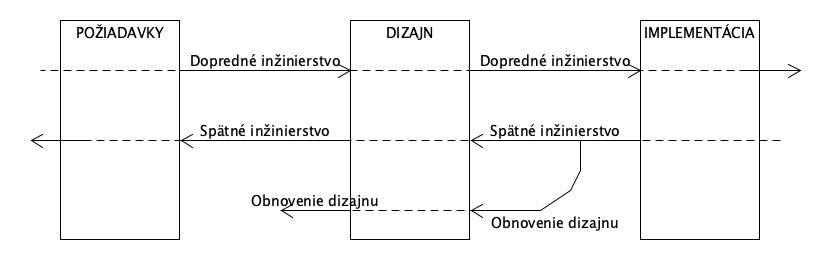
\includegraphics[width=0.85\textwidth]{forward_reverse.jpg}
\caption{Vybrané fázy SDLC a znázornené procesy súvisiace s dopredným a spätným inžinierstvom (prevzaté a preložené z~\cite{2010})}
\label{obr_forward_reverse}
\end{figure}

Spätné inžinerstvo, ako už bolo v sekcii~\ref{klasifikácia} spomenuté, sa snaží pochopiť funkciu systému. Obr. \ref{obr_forward_reverse} ilustruje spôsob vývoja informačných systémov. Pre jednoduchosť boli použité tri fázy životného cyklu, kde prvá -  \emph{"požiadavky"} predstavuje špecifikáciu problému, druhá  - \emph{"dizajn"} zase špecifikáciu riešenia a tretia -  \emph{''implementácia"} predstavuje programovanie a testovanie požadovaného systému.

Pojem dopredné \textit{(forward)} inžinierstvo reprezentuje tradičný proces vývoja softvéru, kedy sa postupuje od prvotných abstraktných modelov, cez dizajn až ku konečnej implementácii systému. Zavedenie názvu pre niečo tak priamočiare sa môže sa zdať zbytočné, možno aj mätúce . V našom prípade, a tiež v mnoho iných, je to však nevyhnutné pre jeho odlíšenie od spätného inžinierstva. Ako teda Obr \ref{obr_forward_reverse} ukazuje, dopredné inžinierstvo prechádza jednotlivými fázami SDLC z ľava do prava.

// Tu príde ešte popis reverzného inžinierstva spolu s odkazovaním sa na obrázok.



\section{Predstavenie nástrojov}\label{predstavenie}

Táto sekcia popisuje nástroje, ktoré boli predmetom skúmania, realizovaného autorom~\cite{Osman:RE}. Všetkých 8 posudzovaných nástrojov je uvedených v tabuľke~\ref{tabulka1}. Pri evaulácii komerčných nástrojov bola použitá verzia pre účely testovania, prípadne verzia na vzedlávacie účely.

%tabulka:
\begin{table}[h]
\centering
\makebox[\textwidth][c]{
\begin{tabular}{|c|p{0.2\textwidth}|c|c|c|}
\hline
č & nástroj CASE & informácie & Predajca & Typ Licencie\\
\hline
1 & Visual \newline Paradigm 8.1 & \href{http://www.visual-paradigm.com/}{Visual Paradigm} & Visual Paradigm & Komerčné\\
\hline
2 & MagicDraw 17.0 & \href{http://www.magicdraw.com/}{MagicDraw} & No Magic & Komerčné\\
\hline
3 & Altova Umodel 2011 & \href{http://www.altova.com/}{Altova Umodel} & Altova& Komerčné\\
\hline
4 & Enterprise \newline Architect 8.0 & \href{http://www.sparxsystems.com.au/}{Enterprise Architect} & Sprax System & Komerčné\\
\hline
5 & Rational \newline Software \newline Architect 8.0.1 & \href{https://www.ibm.com/products/rational-software-architect-designer}{Rational Software} & IBM & Komerčné\\
\hline
6 & MyEclipse \newline 8.6 & \href{https://www.genuitec.com/products/myeclipse/features/}{MyEclipse} & Genuitec & Komerčné\\
\hline
7 & StarUML 5\newline & \href{http://staruml.sourceforge.net/}{StarUML} &StarUML & Open Source\\
\hline
8 & ArgoUML \newline & \href{https://argouml-tigris-org.github.io/tigris/argouml/tours/}{ArgoUML} & Tigris.org & Open Source\\
\hline
\end{tabular}
}
\caption{Zoznam posudzovaných nástrojov (prevzaté a preložené z~\cite{Osman:RE})}
\end{table}

\pagebreak
\section{Porovnanie nástrojov}\label{porovnanie}
 
\section{Zhrnutie} \label{zhrnutie} 
Tento článok skúmal automatizáciu SDLC pomocu nástrojov CASE. Boli uvedené dve rôzne klasifikácie, na základe ktorých možno nástroje CASE rozdeliť. Obe síce vychádzajú z jednotlivých fáz životného cyklu, no jedno delí nástroje podľa konkrétnych fáz a druhé ich zase stručnejšie delí do ranných a neskorých fáz.
V práci je ďalej opísané tzv. \emph{dopredné} inžinierstvo a potreba zavedenia tohto prídavného mena. Neskôr je v článku popísané aj reverzné inžinierstvo a stručne uvedená potreba jeho využitia. 
V posledných častiach sa článok zameriava na ohodnotenie nástrojov CASE v reverznom inžinierstve. Nasledujúce závery, prevzaté od~ \cite{Osman:RE}, boli vyvodené na základe toho, aké schopnosti a funkcie porovnávané nástroje mali.
\emph{// tu pribudne zbytok zhodnotenia práce.}



%\acknowledgement{Ak niekomu chcete poďakovať\ldots}


% týmto sa generuje zoznam literatúry z obsahu súboru literatura.bib podľa toho, na čo sa v článku odkazujete
\bibliography{literatura}
\bibliographystyle{abbrv} % prípadne alpha, abbrv alebo hociktorý iný
\end{document}
